% nam-csound-icsc.tex — ICSC 2026 submission, llncs template
% blind review: keep the Author placeholder until camera-ready
% real repo link + acknowledgements go in at camera-ready
\documentclass[runningheads,a4paper]{llncs}

\usepackage{amssymb}
\setcounter{tocdepth}{3}
\usepackage{graphicx}
\usepackage{tikz}
\usetikzlibrary{positioning,arrows.meta}
\usepackage{pgfplots}
\pgfplotsset{compat=1.17}
\usepackage{hyperref}
\usepackage[margin=1.1in]{geometry}
\hypersetup{hidelinks}
\newcommand{\keywords}[1]{\par\addvspace\baselineskip
\noindent\keywordname\enspace\ignorespaces#1}

\pagestyle{headings}

\begin{document}

\mainmatter

\title{Integrating Neural Amp Modeling into Csound}
\titlerunning{Integrating Neural Amp Modeling into Csound}

% TO GUARANTEE THE DOUBLE BLIND REVIEW PROCESS, KEEP GENERIC NAMES
\author{Author}
% camera-ready: restore \thanks{...} acknowledgement here
\authorrunning{Author}
\institute{InstituteA\\ \email{email@institutedomain.com}}

\maketitle

\begin{abstract}
Neural Amp Modeler (NAM) is the most widely used open-source system for
the black-box modeling of nonlinear audio hardware using neural
networks. A community library of several hundred thousand pre-trained
captures exists, but has yet to be integrated into the Csound ecosystem.
This paper presents \texttt{NAMProcess}, a Csound opcode that performs
real-time NAM inference. The opcode loads standard
\texttt{.nam} model files, switches between models without interrupting audio, adds no algorithmic latency, and runs
comfortably in real time on systems like the Raspberry Pi. A live
dry-referenced volume compensation system built into the opcode holds
every capture in a 25-model test library within $\pm
2$~dB of the player's volume. This paper details the implementation of a thin wrapper around
the NeuralAmpModelerCore C++ library and its integration as a native
plugin opcode, a drag-and-drop Cabbage plugin, and ``tone'' section
of a Raspberry Pi-based guitar pedal.
\keywords{Neural Amp Modeling, Raspberry Pi,
Cabbage Plugin, Opcode, Volume Compensation}
\end{abstract}

\section{Introduction}

Over the past several years a new approach has become standard practice in
guitar audio: record a real device, then train a neural network to
reproduce its input--output behavior. Neural Amp Modeler
(NAM)~\cite{atkinson2025slimmable,nam} is the most widely used
open-source implementation of this approach. Its model format has become standard with over 350,000 captures accumulated on TONE3000 alone~\cite{tone3000} covering a variety of non-linear hardware including amplifiers, effect pedals and preamps, freely downloadable.

\section{Background and Related Work}

Feedforward WaveNet variants and recurrent LSTM networks are the
established black-box models of guitar amplifiers and distortion
circuits, and both run in real
time~\cite{damskagg2019tube,damskagg2019distortion,wright2019rnn,wright2020realtime,wright2020perceptual}.
NAM~\cite{atkinson2025slimmable,nam} packages both architectures behind
a single model format and a training pipeline whose input is a fixed
published reference signal reamped through the target device.

Real-time inference of such models already exists in the other major
environments. RTNeural~\cite{chowdhury2021rtneural} is a general
inference library for audio callbacks, with a SuperCollider UGen and
Max/MSP and Pure Data ports~\cite{pluta_rtneural}. The
\texttt{neural\_tilde} external loads \texttt{.nam} files in
Max/MSP~\cite{neuraltilde}, \texttt{neural-amp-modeler-lv2} embeds the
NAM core in an LV2 plugin~\cite{oliphantlv2}, and anira treats
real-time-safe inference in audio callbacks
generally~\cite{ackva2024anira}. Csound~\cite{lazzarini2016csound} has
no equivalent. Its prior guitar-gear modeling derives from circuit
knowledge rather than data, like the component-level triode stage opcode of
Fink and Rabenstein~\cite{fink2011triode} or Rory Walsh's model of the Ibanez Tube Screamer pedal~\cite{walsh2019tubescreamer}. \texttt{NAMProcess} closes that gap.

\section{The NAMProcess Opcode}
\label{sec:opcode}

\subsection{Interface}
\label{sec:interface}

\begin{verbatim}
aoutL, aoutR NAMProcess ainL, ainR,
      kProfileIdx, SLibDir
      [, kAutoVol]
icount       NAMCount
\end{verbatim}

\texttt{SLibDir} points at a folder, scanned recursively for
\texttt{.nam} files at init. The sorted file list gives every model a
stable index, and \texttt{kProfileIdx} picks one at k-rate. Writing a new index kicks off an asynchronous load, and the running model keeps playing until the new one is ready. \texttt{NAMCount} reports
the library size so orchestra logic can wrap or clamp. Since model
choice is just another k-rate value, modulating high-quality NAM models is now open to the same
rule-based and generative processes Koenig
practiced~\cite{koenig1970project2}.
\texttt{kAutoVol} enables the volume compensation of
Section~\ref{sec:volume}, on by default. A minimal live instrument follows.

\begin{verbatim}
instr 1
  aL, aR  ins
  kIdx    chnget "model" ; MIDI, OSC, score
  aoL,aoR NAMProcess aL, aR, kIdx,
          "/home/user/models"
  outs aoL, aoR
endin
\end{verbatim}

Until the first model loads, or if the folder holds no models, audio
passes through untouched so a misconfigured path degrades to bypass instead of silence.

\subsection{Loader and Model State}
\label{sec:loader}

Everything that touches files or network weights runs on a background
thread owned by the opcode~\cite{bencina2011realtime}. The audio thread never
allocates, parses JSON, or blocks on I/O. Per k-cycle it takes one
uncontended mutex acquisition to copy a pointer to the active model
pair. The loader builds the requested model, picks the full-quality
submodel (for when "slimmable models" are an option)~\cite{atkinson2025slimmable}, and
pre-warms internal buffers before publishing the swap. A failed load
keeps the previous model running, so a corrupt file cannot interrupt a performance, and swaps land on a block boundary to keep audio free of clicks.

A model trained at a different sample rate than the engine gets wrapped
in a Lanczos resampling container so the network always runs at its trained rate. A 48~kHz
model under a 44.1~kHz engine matches the matched-rate reference within 0.3~dB. 

NAM models are stateful. WaveNet layers keep convolution history in ring buffers and LSTMs carry hidden state between calls. So
\texttt{NAMProcess} loads two independent instances of the same file,
resets both off-thread, and publishes them as a pair, one per channel. Running both channels through one shared instance convolves every block against the other channel's immediate past, which measures as $-4.7$~dB crosstalk on decorrelated stereo material.

\subsection{Latency}
\label{sec:latency}

The supported architectures are causal, so the opcode itself should add
no delay. The latency at 128
samples is 2.7~ms at 48~kHz in the pedal deployment of
Section~\ref{sec:pedal}.

\section{Live Volume Compensation}
\label{sec:volume}

The opcode continuously matches the wet output to the perceived loudness
of the player's dry signal, so loading any capture (clean, cranked,
mislabeled) leaves the volume unchanged.

Without this, browsing a community library is impractical live. Fed the
same signal, the 25 representative captures of Fig.~\ref{fig:bench}
span 17~dB even after a load-time normalization probe, and embedded
loudness metadata does not predict the ranking. No pre-computed
correction can close the gap, because saturating models compress: one
compression-dominated capture holds its output within 1~dB across a
14~dB input sweep, so no per-model gain equalizes it at all. The
correction has to be relative to what the player is actually doing live.

Dry input and wet output are metered as ITU-R BS.1770 K-weighted mean
squares averaged with a 2.5~s time constant, and a slow output trim tracks
their ratio (Fig.~\ref{fig:comp}). Neither meter observes the trim's
own effect, so the control loop is feed-forward and cannot oscillate. Program dynamics move both meters together and leave the
ratio untouched to ensure the mechanism does not add any feeling of compression. The goal is a system where loudness is held constant while spectrum and saturation can vary. Measured after convergence, a $-12$~dB input step passes through as $-10.2$~dB of output,
the residual being the amp's own compression. The trim engages after one
second of active signal, slews at most 2~dB/s, holds within a 0.75~dB
deadband, freezes below $-55$~dBFS input, and is clamped to $\pm 18$~dB.
Converged trims are remembered per model file, so returning to a played capture lands at level immediately ($+0.6$~dB measured). 

\begin{figure}
\centering
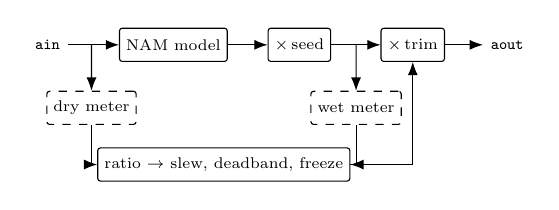
\begin{tikzpicture}[scale=0.8, transform shape,
  box/.style={draw, rounded corners=1pt, minimum height=1.5em,
              inner sep=3pt, font=\scriptsize},
  lbl/.style={font=\scriptsize\ttfamily}, >=Latex]
\node[lbl] (in)    at (0,0)    {ain};
\node[box] (model) at (2.0,0)  {NAM model};
\node[box] (seed)  at (4.0,0)  {$\times$\,seed};
\node[box] (trim)  at (5.8,0)  {$\times$\,trim};
\node[lbl] (out)   at (7.3,0)  {aout};
\node[box,dashed] (dm) at (0.7,-1.0) {dry meter};
\node[box,dashed] (wm) at (4.9,-1.0) {wet meter};
\node[box] (ctl) at (2.8,-1.9) {ratio $\rightarrow$ slew, deadband, freeze};
\draw[->] (in) -- (model);
\draw[->] (model) -- (seed);
\draw[->] (seed) -- (trim);
\draw[->] (trim) -- (out);
\draw[->] (0.7,0) -- (dm);
\draw[->] (4.9,0) -- (wm);
\draw[->] (dm) |- (ctl);
\draw[->] (wm) |- (ctl);
\draw[->] (ctl) -| (trim);
\end{tikzpicture}
\caption{Live compensation topology inside one \texttt{NAMProcess}
cycle. The dry meter taps the raw input and the wet meter taps after the model, before the trim.}
\label{fig:comp}
\end{figure}


\begin{figure}
\centering
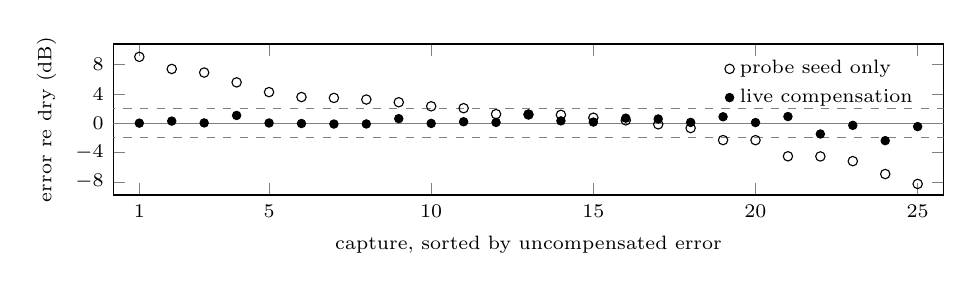
\begin{tikzpicture}
\begin{axis}[width=\linewidth, height=3.5cm,
  xmin=0.2, xmax=25.8, ymin=-9.8, ymax=10.8,
  xlabel={capture, sorted by uncompensated error},
  ylabel={error re dry (dB)},
  label style={font=\scriptsize}, tick label style={font=\scriptsize},
  legend style={font=\scriptsize, draw=none, fill=none,
                at={(0.98,0.97)}, anchor=north east},
  legend cell align=left,
  xtick={1,5,10,15,20,25}, ytick={-8,-4,0,4,8}]
\addplot[gray, thin, domain=0:26, samples=2] {0};
\addplot[gray, thin, dashed, domain=0:26, samples=2] {2};
\addplot[gray, thin, dashed, domain=0:26, samples=2] {-2};
\addplot[only marks, mark=o, mark size=1.7] coordinates {(1,9.04) (2,7.39) (3,6.90) (4,5.56) (5,4.23) (6,3.56) (7,3.44) (8,3.22) (9,2.85) (10,2.30) (11,2.04) (12,1.23) (13,1.18) (14,1.13) (15,0.74) (16,0.38) (17,-0.16) (18,-0.67) (19,-2.31) (20,-2.32) (21,-4.52) (22,-4.54) (23,-5.18) (24,-6.94) (25,-8.29)};
\addplot[only marks, mark=*, mark size=1.5] coordinates {(1,0.00) (2,0.28) (3,0.03) (4,1.05) (5,0.02) (6,-0.05) (7,-0.12) (8,-0.11) (9,0.61) (10,-0.04) (11,0.19) (12,0.10) (13,1.20) (14,0.31) (15,0.15) (16,0.68) (17,0.57) (18,0.10) (19,0.87) (20,0.08) (21,0.90) (22,-1.48) (23,-0.30) (24,-2.39) (25,-0.47)};
\legend{,,,probe seed only,live compensation}
\end{axis}
\end{tikzpicture}
\caption{Loudness error relative to the dry input, all 25 captures on
identical material (saw plucks, peak 300~ms RMS, settled), sorted by uncompensated error. Dashed lines mark $\pm 2$~dB.}
\label{fig:bench}
\end{figure}

Figure~\ref{fig:bench} measures the shipped system: the live loop
collapses the 17.3~dB seed-only spread (standard deviation 4.3~dB) to
3.6~dB (0.74~dB), all but one capture within $\pm 2$~dB of the dry
signal, including the compression-dominated capture that no input
gain can equalize. On the guitar material used during development the
corresponding spread is 3.1~dB (0.83~dB), every capture inside $\pm 2$~dB. The best purely static probe evaluated left 9.9~dB (2.60~dB). The official NAM plugin's normalized output mode~\cite{namplugin} applies a static gain from stored metadata or a fixed target.
To my knowledge, no published NAM host performs live dry-referenced
compensation.

\section{A Drag-and-Drop Cabbage Plugin}
\label{sec:plugin}

This opcode is accessible as a VST3/AU plugin through
Cabbage~\cite{walsh2011cabbage}. Cabbage publishes the
dropped file's path on its \texttt{LAST\_FILE\_DROPPED}
channel, and a path-input loader variant hot-swaps to it through the
background mechanism of Section~\ref{sec:loader}. The UI reports the loaded model, but provides arrows 
to navigate other NAM files in the same parent folder. The compensation of Section~\ref{sec:volume} defaults on, but can be toggled off exposing raw model level. The input and output knobs are clean gains in dB. The input gain feeds both the model and the dry reference of the compensation, so it acts as plain volume while the model supplies the saturation. A gate, three-band tone stack,
and DC blocker mirror the outboard chain of the official NAM plugin~\cite{namplugin}. An orchestra that fails to compile emits silence yet passes host validation, so the
base orchestra contains no NAM references and the engine instrument is
compiled at runtime with \texttt{compilestr}. If
the opcode library fails to load, audio passes through dry and the failure
is reported on the status display.

\section{Raspberry Pi Guitar Pedal}
\label{sec:pedal}

The opcode's original deployment target is a Raspberry Pi 5-based
guitar pedal running Csound 6.18 at 48~kHz with \texttt{ksmps} 128. The
audio chain pinned to one dedicated core, where the 25-capture library
acts as a bank of ``tones''. Model selection is mapped to MIDI foot
controls. Loading is
click-safe and volume matched so the player can smoothly switch between amps mid-performance. The only added latency is the block granularity
of Section~\ref{sec:latency} (2.7~ms), well inside a live monitoring
budget. CPU load with only a full-quality NAM model running has been informally
observed around 15\% of the audio core during performance.

\section{Conclusions}
\label{sec:conclusions}

\texttt{NAMProcess} gives Csound direct access to NAM's model format
and community library as a drop-in nonlinear processor addressable by a
k-rate index, shipping as a Cabbage plugin and a Raspberry Pi implementation. Source code and measurement tooling
will be released under an open-source license upon publication.

\begin{thebibliography}{21}

\bibitem{ackva2024anira} Ackva, V., Schulz, F.: anira: An Architecture
for Neural Network Inference in Real-Time Audio Applications. In:
Proceedings of the 5th IEEE International Symposium on the Internet of
Sounds (IS2) (2024)

\bibitem{atkinson2025slimmable} Atkinson, S.: Slimmable NAM: Neural Amp
Models with Adjustable Runtime Computational Cost. arXiv:2511.07470 (2025)

\bibitem{nam} Atkinson, S.: Neural Amp Modeler and NeuralAmpModelerCore,
\url{https://www.neuralampmodeler.com},
\url{https://github.com/sdatkinson/NeuralAmpModelerCore}

\bibitem{namplugin} Atkinson, S.: Neural Amp Modeler Plugin, \url{https://github.com/sdatkinson/NeuralAmpModelerPlugin}

\bibitem{bencina2011realtime} Bencina, R.: Real-time Audio Programming
101: Time Waits for Nothing,
\url{http://www.rossbencina.com/code/real-time-audio-programming-101-time-waits-for-nothing}

\bibitem{chowdhury2021rtneural} Chowdhury, J.: RTNeural: Fast Neural
Inferencing for Real-Time Systems. arXiv:2106.03037 (2021)

\bibitem{damskagg2019tube} Damsk\"agg, E.-P., Juvela, L., Thuillier, E.,
V\"alim\"aki, V.: Deep Learning for Tube Amplifier Emulation. In:
Proceedings of the IEEE International Conference on Acoustics, Speech and
Signal Processing (ICASSP), pp. 471--475. Brighton (2019)

\bibitem{damskagg2019distortion} Damsk\"agg, E.-P., Juvela, L.,
V\"alim\"aki, V.: Real-Time Modeling of Audio Distortion Circuits with
Deep Learning. In: Proceedings of the 16th Sound and Music Computing
Conference (SMC), pp. 332--339. M\'alaga (2019)

\bibitem{fink2011triode} Fink, M., Rabenstein, R.: A Csound Opcode for a
Triode Stage of a Vacuum Tube Amplifier. In: Proceedings of the 14th
International Conference on Digital Audio Effects (DAFx-11), pp. 365--370.
Paris (2011)

\bibitem{koenig1970project2} Koenig, G.M.: Project 2: A Programme for
Musical Composition. Electronic Music Reports 3. Institute of Sonology,
Utrecht State University, Utrecht (1970)

\bibitem{lazzarini2017cpof} Lazzarini, V.: The Csound Plugin Opcode
Framework. In: Proceedings of the 14th Sound and Music Computing
Conference (SMC), pp. 267--274. Espoo (2017)

\bibitem{lazzarini2016csound} Lazzarini, V., Yi, S., ffitch, J., Heintz,
J., Brandtsegg, {\O}., McCurdy, I.: Csound: A Sound and Music Computing
System. Springer, Cham (2016)

\bibitem{oliphantlv2} Oliphant, M.: neural-amp-modeler-lv2,
\url{https://github.com/mikeoliphant/neural-amp-modeler-lv2}

\bibitem{pluta_rtneural} Pluta, S.: RTNeural Real-Time Neural Inference
UGen, \url{https://scsynth.org/t/rtneural-real-time-neural-inference-ugen/10074}

\bibitem{neuraltilde} Presta, A.: neural\_tilde: Neural Amp Modeler
External for Max/MSP, \url{https://github.com/apresta/neural_tilde}

\bibitem{tone3000} TONE3000, \url{https://www.tone3000.com}

\bibitem{walsh2011cabbage} Walsh, R.: Developing Csound Plugins with
Cabbage. In: J. Heintz, A. Hofmann, I. McCurdy (eds.) Ways Ahead:
Proceedings of the First International Csound Conference. Cambridge
Scholars Publishing, Newcastle upon Tyne (2013)

\bibitem{walsh2019tubescreamer} Walsh, R., Walsh, C.: Digital Signal
Processing Techniques Used to Model the Ibanez Tube Screamer Guitar
Pedal. In: Proceedings of the 5th International Csound Conference
(ICSC 2019). Cagli (2019)

\bibitem{wright2019rnn} Wright, A., Damsk\"agg, E.-P., V\"alim\"aki, V.:
Real-Time Black-Box Modelling with Recurrent Neural Networks. In:
Proceedings of the 22nd International Conference on Digital Audio Effects
(DAFx-19), pp. 173--180. Birmingham (2019)

\bibitem{wright2020realtime} Wright, A., Damsk\"agg, E.-P., Juvela, L.,
V\"alim\"aki, V.: Real-Time Guitar Amplifier Emulation with Deep
Learning. Applied Sciences 10(3), 766 (2020)

\bibitem{wright2020perceptual} Wright, A., V\"alim\"aki, V.: Perceptual
Loss Function for Neural Modelling of Audio Systems. In: Proceedings of
the IEEE International Conference on Acoustics, Speech and Signal
Processing (ICASSP), pp. 251--255. Barcelona (2020)

\end{thebibliography}

\end{document}
